\section{서론}

매년 이루어지는 통계청의 사회조사에서 세대 간 계층이동성에 대한 설문에 대한 응답은 2000년대 이후 현재까지 매우 빠른 계층이동에 대한 인식의 변화를 보여준다.\footnote{본 연구는 \citet{onj20}로 출간된 바 있다.}
그러나 교육부의 2017년 설문조사에 따르면(교육부(2017), “경제⋅사회 양극화에 대응한 교육복지 정책의 방향과 과제”) 응답자의 93.9\%가 계층 간 교육격차가 크다고 응답하였고, 87\%가 과거에 비해 교육격차가 커졌다고 인식하여 계층사다리로서의 교육의 역할이 부실한 것이 세대 간 계층이동에 대한 전망의 주요 원인으로 지목되고 있다.
위 교육부 설문조사에서 교육격차의 가장 큰 원인으로 67.7\%가 교육비 격차라고 응답하였는데 실제 가계동향조사에 따르면 월 소득 600만원 이상 가정과 100만원 미만 가정의 교육비 지출 격차가 2016년 10.2배, 사교육비의 경우 12.7배에 이르는 것으로 나타났다.
대학입시와 초중등 학업성취도 자료를 이용한 여러 연구(가령, \citet{kim11}, \citet{knl08}, \citet{ketl14}, \citet{ohetl16})들이 계층 간 높은 교육격차를 보고하였고 그 원인으로 사교육비의 격차와 사교육비에 영향을 미치는 가구의 사회경제적 지위를 들고 있다.
  
계층 간 교육격차의 해소를 위해 최근 대학입시전형에서 정시 비중을 높이고 고교평준화를 강화하는 방향의 정책이 추진되고 있고 이에 대한 찬반론이 대립되고 있다.
특히 정시와 수시의 공정성 비교에 있어서 교육 및 입시 전문가들의 의견대립이 첨예하다.
본 연구는 대학입시를 둘러싸고 우리 사회의 계층 간 교육격차 혹은 교육 기회불평등의 실태를 분석하고 입시 전형 별 교육기회불평등을 비교하는 것을 목적으로 한다.
이를 바탕으로 최근 추진되고 있는 정시확대 정책의 효과에 대한 정책적 시사점을 도출할 것이다.
  
대부분의 현대 민주주의 국가에서는 인종, 성, 성장환경(부모의 사회경제적 배경, 출신지역 등), 종교 등과 같이 개인의 선택과 무관하게 타고난 환경 요인이 개인의 성취에 영향을 미쳐서는 안 된다는 기회균등의 원칙에 대한 높은 수준의 사회적 합의가 존재한다.
이처럼 기회균등이 요구되는 요인들을 (기회균등)기저요인이라 부를 것이다.
기회불평등에 대한 \citet{letl08, letl09}의 실증적 방법론에 따라, 기저요인의 정량적 크기 혹은 범주에 따라 “환경”을 구분하고 환경 별 성취도의 (조건부) 확률분포를 비교하여 확률분포 간에 제1차 (혹은 제2차) 확률지배관계가 존재할 때 기회불평등이 존재한다고 정의한다.
   
본 연구에서 고려할 기저요인은 부모의 사회경제적 배경, 출신지역, 그리고 성 이다.
각 기저요인에 따른 기회불평등의 존재 유무와 기회불평등도의 추세에 대해 분석할 것이다.
본 연구와 동일한 방법을 활용하여 교육과 소득의 기회불평등에 대해 연구한 선행연구로 \citet{letl08, letl09}, \citet{ohetl16}, \citet{onj17}, \citet{snj21} 등이 있다.
특히 \citet{ohetl16}은 대학입학수학능력평가 자료를 활용하여 가구환경 간 교육기회불평등을 연구하였다.
교육기회불평등에서 가장 중요한 교육성취가 대학입학성과라는 것은 부인하기 어려운 사실이다.
본 연구는 대학입학 성과를 바탕으로 가구환경 간 교육기회불평등을 분석한다는 점에서 차별성이 있다.
   
이 밖에 교육 혹은 소득의 계층 간 기회불평등에 대한 대다수의 선행연구들은 교육 혹은 소득의 성취에 미치는 다양한 요인들을 바탕으로 회귀모형을 설정하고 계수 추정을 통하여 가구환경, 성, 지역 등의 환경요인의 영향을 분석한다(관련 선행연구\citet{knl08} ,\citet{kim11} \citet{kim11}, \citet{ketl14} 등 참고).
이 연구들은 환경요인이 성취에 미치는 평균적 영향을 잘 보여주는 장점이 있으나 평균 이외에도 기회불평등과 관련된 성취 분포의 다른 특성들 (가령 최상위 성취의 가능성, 최하위 성취의 가능성, 성취 위험 등)에 미치는 영향까지 분석하지 않는 경우가 대부분이다.
바로 이점이 본 연구가 갖는 차별성이라 할 수 있다.
   
본 연구는 한국고용정보원의 대졸자직업이동경로(GOMS) 자료를 활용하여 2000년대 초반에서 2010년대 초반에 이르기까지의 기간 동안 매년 가구환경, 성, 지역환경 등이 고교졸업자들의 대학입학 성과 미치는 영향을 분석할 것이다.
이를 통하여 계층별, 성별, 지역별 교육기회불평등의 유무와 기회불평등도의 추세를 도출하고 정시와 수시 각 전형별 기회불평등도와 추세를 비교 검토할 것이다.
대부분의 교육자료는 종단연구(panel study) 형태로 되어 각 자료당 대학입시와 같은 교육성과는 자료조사기간 전체에 한 번 밖에 관찰되지 않는다.
따라서 교육성취와 관련된 연구의 수행에서 매년 추세를 연구할 수 없는데 본 연구가 갖는 두 번째 차별점은 여기에 있다.


\section{기회불평등과 기회불평등 지수}
개인의 성취는 자신의 노력뿐만 아니라 인종, 성, 부모의 사회경제적 지위 등과 같은 환경, 선천적인 재능 그리고 다양한 운에 따라 결정된다.
기회균등이 요구되는 환경들의 집합이 $C$로 주어져 있고 이를 기회균등기저(equal opportunity basis)라 하자.
기회균등 기저에 속한 임의의 환경 $c$에서 노력과 다른 우연적인 요인들에 따라 결정되는 성취 $y$의 확률분포 $y=F(y|c)$를 얻을 수 있다.
바로 이런 조건부 확률분포가 기회균등 기저의 모든 환경들 간에 동일해야 한다는 것으로 강한 기회평등을 정의할 수 있을 것이다.
즉 임의의 두 환경 $c,c' \in C$에 대해 $F(\cdot | c) = F(\cdot | c')$가 성립한다는 의미이다.

그러나 이처럼 강한 기회평등을 요구하는 것은 매우 비현실적이다.
서로 다른 환경이 상이한 성취의 확률분포를 가지더라도 어느 하나가 다른 하나보다 우월하지 않다면 기회평등이 침해되었다고만 볼 수는 없다.
우리는 \citet{letl08, letl09}이 제시한 보다 완화된 기회평등 개념을 활용하여 기회불평등에 대한 분석을 진행할 것이다.

\citet{letl08, letl09}의 기회평등은 어떤 환경도 그 확률분포가 다른 환경의 확률분포를 확률지배하지 않을 경우에 성립한다.
 상이한 두 환경 와 에서 개인의 성취는 각각 와 의 확률분포를 이룬다고 가정하자.
만약 성취 $y$가 취할 수 있는 모든 성취수준 $x$에 대하여, 부등식
\begin{equation}
    F(x | c) \leq F(x | c')
    \label{eq:fdom}
\end{equation}
이 성립하면 환경 $c'$에서 일정수준 이하의 낮은 성취를 이룰 확률이 다른 환경 $c$에서 보다 크다는 것을 의미한다.
 이는 성취의 전망의 관점에서 환경 $c'$이 환경 $c$보다 열악하다는 것이다.
 이처럼 모든 성취수준에서 식 (\ref{eq:fdom})이 성립하고 적어도 하나의 성취수준에서 이 부등식이 강부등식으로 성립할 때 환경 $c$가 환경 $c'$을 제1차 확률지배한다고 말한다.

만약 모든 성취수준 $x$에서, 부등식
\begin{equation}
   \int_{0}^{x} F(y | c)\,dy \leq \int_{0}^{x} F(y | c')\,dy
    \label{eq:sdom}
\end{equation}
이 성립하고 적어도 하나의 성취수준에서 이 부등식이 강부등식으로 성립할 때 환경 $c$가 다른 환경 $c$을 제2차 확률지배한다고 말한다.
이 경우 성취에 대한 위험기피적인 선호를 가진 사람은 항상 환경 $c$의 확률분포를 선호하게 된다.

기회균등기저에 속한 어떤 두 환경 간에 제1차 혹은 제2차 확률지배관계가 존재할 경우 기회불평등이 존재한다고 정의한다. 

제1차 기회불평등 조건: 어떤 두 환경 $c,c' \in C$에 대하여 $F(y | c)$와 $F(y | c')$사이에 제1차 확률지배관계가 성립한다.

제2차 기회불평등 조건: 어떤 두 환경 $c,c' \in C$에 대하여 $F(y | c)$와 $F(y | c')$사이에 제2차 확률지배관계가 성립한다.

그리고 기회평등은 이러한 기회불평등이 존재하지 않는 경우에 성립한다.
따라서 본 논문에서 기회평등한 사회는 기회균등기저에 속한 서로 다른 환경들이 상이한 성취의 기회(확률분포)를 제공할 수 있다.
단, 어느 환경도 다른 환경보다 더 확률지배적인 성취의 기회를 제공해서는 안 될 뿐이다.
 
보다 근본적으로 환경뿐만 아니라 개인의 노력도 기회불평등을 정의함에 있어서 고려되어야 한다(\citet{Roemer98}; \citet{letl08, letl09}).
즉, 동일한 노력을  한 사람들에게 환경의 기회격차가 존재해서는 안된다는 기회평등은 설득력을 가질 수 있지만 노력을 더 많이 한 사람에게 더 좋은(확률지배적) 기회가 보장되는 것을 불공정하다고 볼 수 없는 것이다.
이처럼 환경뿐만 아니라 노력의 크기까지도 조건화하여 위에서 말한 확률지배관계를 정의하고 이를 이용하여 기회불평등을 정의하는 것이 보다 근본적인 접근이라 할 수 있다.
이러한 접근법을 택하더라도 개인의 노력을 ``순수한'' 노력변수로 나타낸다면 결과적으로 앞서 정의된 노력이 고려되지 않은 기회불평등 조건이 필요조건이 될 수밖에 없다.
여기서 노력이 순수하다는 것은 노력의 분포 자체도 환경의 영향을 받지 않는다는 것을 의미한다.
이와 관련하여 보다 자세한 논의는 선행연구인 \citet{Roemer98}, \citet{letl08, letl09}, 오성재외(2016), 오성재·주병기(2017) 등에 잘 소개되어 있다.

두 기회불평등 조건에 나타난 확률지배관계 검증은 \citet{dnd00}의 비모수 검증법을 활용한다.
먼저 기회균등기저의 환경을 기준으로 집단을 나누고 환경별 성취의 누적분포함수 $F(y | c)$를 얻는다.
이렇게 얻어진 환경별 분포함수들 간에 확률지배관계 성립 여부를 검증하는 것이다.
우선 임의의 두 환경 $c,c'$사이에 $F(y | c)$가 $F(y | c')$을 1차(2차) 확률 지배를 하고 그 역은 성립하지 않을 경우 전자가 후자를 1차(2차) 확률지배하는 것으로 확인된다.
이처럼 확률지배관계가 확인되지 않을 경우 두 분포의 동일성 여부를 검증하는 순서로 진행된다.

확률지배검증은 기회불평등의 존재 유무만을 알려준다.
그러나 똑같이 기회불평등한 사회 간에도 기회불평등의 크기를 비교하려면 기회불평등 지수가 필요하다.
\citet{letl08}은 불평등 지수로 널리 쓰이는 지니계수에서 착안한 지수를 활용하였다.
환경 $t$의 평균성취수준을 $\mu _t$, 불평등도(지니계수)를 $G _t$라고 할 경우, 환경 $t$에서의 성취기회의 ``가치''는 $\mu _t (1-G _t)$로 나타낼 수 있을 것이다.
즉, 평균성취수준이 클수록 그리고 불평등도가 낮을수록 환경 $t$의 성취기회의 가치는 상승하는 것이다.
\footnote{\citet{yitzhaki79}는 $\mu _t (1-G _t)$를 환경 $t$에 속하는 개인들이 자신의 환경에 대하여 가지는 상대적 만족감이라고 한다.}
모든 환경에 대하여 이렇게 환경의 가치를 측정하고 이러한 가치 값들에 대한 불평등도를 다시 지니계수로 구한 것이 지니(Gini) 기회불평등지수(혹은, GO 지수)이다.
총 $k$개의 환경이 있고 환경 가치의 평균값을 $\mu$라고 하면, 각 환경 $t$의 비중이 $P_t$일 때, 지니 기회불평등지수는 다음 식과 같이 정의된다.

\begin{equation}
    G O=\frac{1}{\mu} \sum_{i=1}^{k} \sum_{j>i} P_{i} P_{j}\left(\mu_{j}\left(1-G_{j}\right)-\mu_{i}\left(1-G_{i}\right)\right).
    \label{eq:goms_GOI}
\end{equation}

열악한 환경에서도 최상위 성취전망이 높은 사회에서는 계층상승의 기회가 크다고 할 수 있다.
이처럼 최하위에서 최상위로의 계층상승의 전망을 반영하는 지표도 기회불평등지표로 유용하게 활용될 수 있다.
가장 열악한 환경 $\underline{c}$에 처한 사람들의 전체인구에서의 비율을 $q_{\underline{c}}$이라 하자.
최상위 성취 집단을 소득 상위 $p$퍼센트에 속하는 사람들이라고 하고 이들의 수를 $n_p$라고 하자.
 
그리고 이들 중 가장 열악한 환경 $\underline{c}$에 처한 사람들의 $n_{p,\underline{c}}$수를 라고 하면, 개천용(기회)불평등지수(혹은, RR 지수)는 최상위 성취집단에서 최하위 환경의 비율을 이용하여 다음과 같이 정의된다
\footnote{개천용불평등지수는 본 연구와 동시에 진행된 교육기회불평등에 대한 연구인 오성재外(2017)에서도 소개된 바 있다.}
\begin{equation}
    R R_{p}=1-\frac{n_{p, \underline{c}} / n_{p}}{q_{\underline{\underline{c}}}} .
    \label{eq:goms_RRI}
\end{equation}
개천용불평등지수 값이 0이라는 것은 최상위 성취를 이룬 사람들 중에서 최하위 환경을 가진 사람들의 비율이 최하위 환경 사람들의 인구비율과 동일하다는 것을 의미하고 이는 기회불평등이 없는 상태를 나타낸다.
 개천용불평등지수 값이 1이라는 것은 반대로 최상위 성취를 이룬 사람들 중에서 최하위 환경을 가진 사람이 없다는 것을 의미하고 이는 기회불평등도가 가장 높은 상태를 나타낸다.
 개천용불평등지수 값이 음이 되는 경우도 있는데 이는 최하위 환경이 최상위 성취를 달성하는데 오히려 유리한 ``역''기회불평등의 상태를 말한다.

개천용불평등지수가 0인 사회에서는 가장 열악한 환경에서도 다른 환경과 동일한 확률로 성공이 보장된다고 볼 수 있다.
개천용불평등지수가 양수 의 값을 가진다면 최악의 환경에서 성공할 수 있는 100명 중에서 $100 \times q$명(퍼센트)가 기회불평등 때문에 성공하지 못하는 것으로 볼 수 있다.
예를 들어 개천용불평등지수가 0.6인 사회에서는 최악의 환경에서 성공할 수 있는 100명중에서 60명이 기회불평등 때문에 실패하게 되는 것이다.
\footnote{본 연구에서는 성공의 기준을 최상위 등급의 대학진학으로 정의한다.}


\section{분석자료}
대졸자직업이동경로조사(이하 GOMS)는 한국고용정보원 주관으로 2005년부터 집계된 반복 횡단면 자료이다.
목표 모집단은 조사시점 최근 1년간 전국의 모든 대학졸업자이고 이 가운데 약 4\%에 해당하는 18,000명을 조사하고 있다.
 (비)경제활동상황, 일자리상태, 학교생활, 취업준비, 인적사항 등의 정보를 수집하고 있다.
 최초구상은 2005년부터 조사하는 종단면 자료로 계획되었으나, 예산문제로 2006년 조사가 시행되지 못했다.
 2007년부터 매 해 1차 조사 및 2년 후 1회 추적조사를 실시하는 것으로 변경되었고, 2012년부터는 매 해 1차 조사만 시행하고 있다.
 본 연구는 2007년부터 2017년까지의 1차 조사 자료를 반복된 횡단면 자료로 활용하였다.

\begin{figure}
    \centering
    \caption{고교졸업년도별 관측치}
    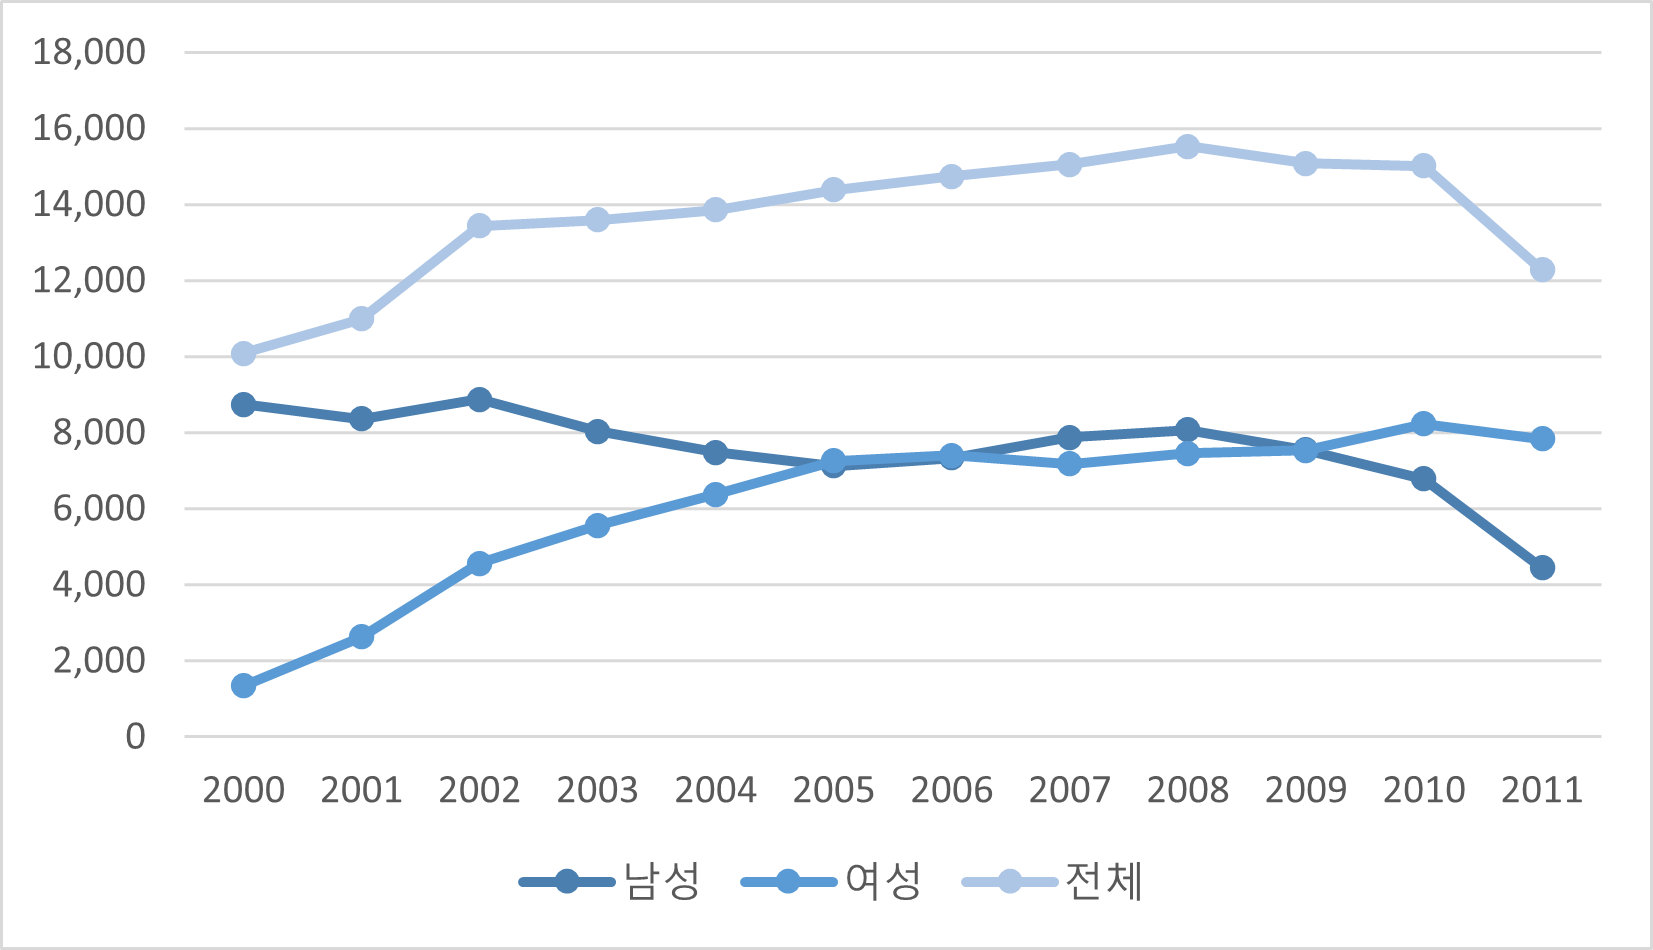
\includegraphics[width=\textwidth]{figure/goms_gender.png}
    \label{fig:goms_gender}
\end{figure}

GOMS의 모집단은 최근 1년 이내의 대학 졸업자들이다.
이들을 고교졸업년도를 기준으로 2000년에서 2011년까지 총 12개 코호트로 분류하였다.
 1999년 이전과 2012년 이후의 경우 코호트 집단의 학생 수가 크게 줄어들어 분석에서 제외하였다(그림 \ref{fig:goms_gender}참조).

군 복무 문제로 남학생과 여학생의 성비가 자료의 초기와 말기에 큰 불균형이 발생하는 것을 피하기 어렵다.
또한 자료의 초기에는 대학교육 연수가 평균보다 긴 학생들이 더 많은 비중을 차지하고 말기에는 반대로 이런 학생들의 비중이 줄어드는 문제도 존재한다는 것을 염두에 둘 필요가 있다.
대체로 성비 균형을 보이는 코호트는 2004년에서 2009년까지이다.
2004년 이전 코호트에는 여성이 과소 집계되었고 2010년 이후에는 남성이 과소 집계되었다.
그러나 성별 기회불평등이 미미하다는 점을 고려할 때 이러한 성비의 문제는 분석에 큰 영향이 없을 것이라 짐작한다.

교육성취는 졸업자들의 졸업대학 및 전공 정보와 2019년 QS 대학순위를 결합하여 1점에서 5점까지로 점수화하였다.
먼저 QS순위기준 최상위 대학 및 전국의 의, 치, 한, 수의대 및 약대에 5점을 부여하였다. 다음으로 QS순위 최상위를 제외환 10위까지의 대학은 4점, QS 순위 11-49위 및 전국의 교육대학은 3점, 그 밖의 4년제 대학은 2점, 그리고 2-3년제 대학은 1점을 부여하였다. 

기회균등기저에는 부친 및 모친의 학력과 부모의 대학입학당시 소득, 성, 그리고 출신고교의 소재지와 같은 환경변수를 포함시켰다.
또한 부모 학력과 소득을 이용한 주성분분석에서 얻어진 가구환경지수를 환경변수로 포함하였다. 
부친의 학력과 모친의 학력은 무학에서 대학원까지 7개로 각각 분류되어 있는데 이를 단순 합하여 2-14까지 범주로 구성하였고 이를 코호트별로 3등분에 가깝게 저, 중, 고 세 수준으로 나눠 기회불평등에 대한 분석을 진행하였다. 
부모의 소득은 8개 문항으로 조사되었는데 최저가 월소득 100만원 미만이고 최고가 월소득 1000만원 이상이다.
문항의 결과를 부모교육환경과 마찬가지로 코호트 기준 3등분에 가깝게 저, 중, 고 세 수준으로 나눴다. 
부모의 소득은 주로 중위가 많고 학력의 경우 고졸의 수가 전체에서 차지하는 비중이 높다.
이에 더해 소득은 경제성장에 의해 매년 상승하고, 과거 교육기회의 확대에 의해 매년 학부모의 교육수준 역시 급격하게 상승한다.
따라서 이를 코호트별로 세 집단으로 분할할 경우 각 집단의 비율을 동일하게 유지하기 어렵다.
이 뿐만 아니라 고교생의 교육적 성취에 영향을 미치는 성장가구의 환경변수를 얻는데 부모의 학력과 소득를 모두를 집계하는 것이 보다 적절하다 할 수 있다.
따라서 부모의 학력과 소득을 주성분분석(Principal Component Analysis)을 통해 단일변수로 집계하였고 집계된 가구환경지수 값의 분포를 3등분에 가깝게 저, 중, 고 세 가구환경으로 나눴다.
 
성장지역환경은 출신고교의 소재지를 기준으로 서울, 경기 일부지역 및 인천을 수도권, 나머지 광역시 및 세종시를 광역시권, 수도권 이외의 경기도 지역과 나머지 도 단위 및 제주도를 도지역권으로 나눴다.
\footnote{서울과 인접하고 인구가 많은 고양시, 광명시, 부천시, 성남시, 수원시, 안산시, 안양시, 용인시, 의정부시를 수도권에 포함했다.}

 한국의 자료를 이용한 기회불평등 분석에서 환경유형의 구분은 주의해야 한다. 우리 사회는 60년대 이후 산업구조와 교육기회 양자에서 급격한 진보를 경험했다. 그 결과 개인들의 부모의 학력 또는 직업력을 이용해 환경유형을 구분할 경우, 그 구성비가 시계열적으로 계속 변화한다.
 <그림 \ref{fig:goms_nratio_byedu}>은 각 코호트별 부친의 학력을 기준으로 할 경우의 구성비다.
  2000년 코호트는 초대졸 이상이 31.79\%인데 이 비율은 졸업년별로 지속적으로 증가하여 2011년 코호트는 46.80\%가 초대졸이상의 학력을 가진 부친을 두게 된다.
 \footnote{조사대상의 부모가 대학을 입학했던 시점인 1981년을 기준으로 정부 정책에 의해 대학교 신입생 정원이 1년만에 20만명대에서 30만명대로 10만명 가량 증가하였다.}
고졸부친은 전체 코호트에서 44\% 근처로 일정하지만 초대졸 이상의 비율이 늘어나는 만큼 중졸이하의 비중이 15\% 가량 줄어든다. 따라서 부모의 학력을 기준으로 환경을 세 가지 유형으로 분리할 경우 코호트별로 환경유형의 구성이 계속 바뀐다.
c
\begin{figure}
    \centering
    \caption{부친학력기준 자료비율}
    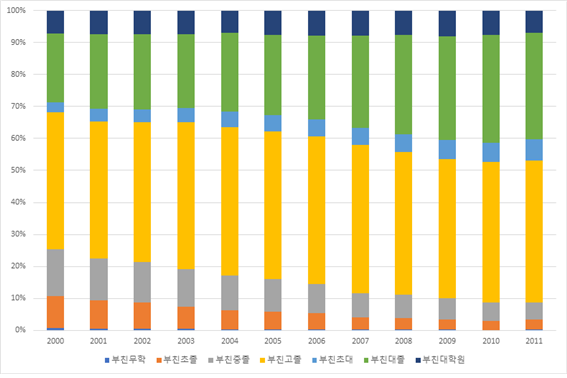
\includegraphics[width=\textwidth]{figure/goms_nratio_byedu.png}
    \label{fig:goms_nratio_byedu}
\end{figure}

이 문제는 주성분 분석(Principal Component Analysis) 기법을 통해 해결하였다.
<그림 \ref{fig:goms_pca}>의 오른쪽은 부친의 학력, 모친의 학력, 부모의 소득 세 변수를 설명변수로 하는 주성분점수의 값의 코호트별 분포이다.
 <그림 \ref{fig:goms_nratio_byedu}>과 같이 범주화된 점수와 비교했을 때, 개인에게 할당된 주성분 점수는 상당히 연속적임을 알 수 있다.
 <그림 \ref{fig:goms_pca}>의 왼쪽은 코호트별로 주성분 점수를 3등분 하여 저, 중, 고유형으로 범주화 한 비율의 히스토그램이다.
 점선은 $1/3$ 값인데 코호트별로 환경유형이 고르게 분할되었음을 알 수 있다.

\begin{figure}
    \centering
    \caption{코호트별 주성분점수(우)와 주성분분석환경 구성비율(좌)}
    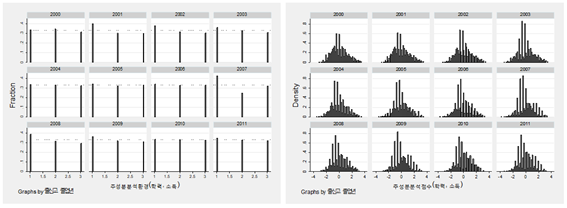
\includegraphics[width=\textwidth]{figure/goms_pca.png}
    \label{fig:goms_pca}
\end{figure}

어떤 대학입시 유형이 공정한가는 교육의 기회와 관련하여 최근 주목받는 주제이다.
이를 분석하기 위해 본 자료에서 제공되는 개인들이 응시한 대입유형 변수를 활용하여 일반 정시, 일반 수시, 특별전형 및 기타로 나누었다.
 일반 정시는 정시, 수능 위주, 논술 위주 및 실기 위주 입시를 포함하고 일반 수시는 수시, 학생부종합 및 학생부교과 위주의 전형을 포함한다.
 특별전형 및 기타는 수시, 정시와 관계없이 정원외 정원 등의 특별전형을 포함하는데 이들은 입시유형별 분석에서는 제외하였다.

\begin{table}[htbp]
    \centering
    \caption{학년도별 대입정원의 정시$\cdot$수시 구성}
    \resizebox{\textwidth}{!}{
\begin{tabular}{c|c|c|c|c|c|c|c}
\hline 학년 & 수시 $^{*}$ & 수시비율 $^{*}$ & 정시 $^{*}$ & 정시비율 $^{*}$ & 합계 $^{*}$ & 수시비율 & 정시비율 \\
\hline 2002 & 107,821 & $28.8 \%$ & 266,063 & $71.2 \%$ & 373,884 & $12.6 \%$ & $81.5 \%$ \\
\hline 2003 & 112,667 & $29.3 \%$ & 271,359 & $70.7 \%$ & 384,026 & $17.1 \%$ & $78.1 \%$ \\
\hline 2004 & 155,941 & $38.5 \%$ & 248,995 & $61.5 \%$ & 404,936 & $24.1 \%$ & $71.1 \%$ \\
\hline 2005 & 174,979 & $44.4 \%$ & 219,400 & $55.6 \%$ & 394,379 & $29.7 \%$ & $65.6 \%$ \\
\hline 2006 & 188,213 & $48.3 \%$ & 201,371 & $51.7 \%$ & 389,584 & $32.0 \%$ & $63.6 \%$ \\
\hline 2007 & 194,442 & $51.5 \%$ & 183,021 & $48.5 \%$ & 377,463 & $34.5 \%$ & $60.3 \%$ \\
\hline 2008 & 200,878 & $53.1 \%$ & 177,390 & $46.9 \%$ & 378,268 & $35.4 \%$ & $58.8 \%$ \\
\hline 2009 & 214,481 & $56.7 \%$ & 163,996 & $43.3 \%$ & 378,477 & $34.8 \%$ & $58.2 \%$ \\
\hline 2010 & 219,024 & $57.9 \%$ & 159,117 & $42.1 \%$ & 378,141 & $34.9 \%$ & $56.8 \%$ \\
\hline 2011 & 232,781 & $60.7 \%$ & 150,761 & $39.3 \%$ & 383,542 & $37.9 \%$ & $52.6 \%$ \\
\hline
\end{tabular}}
    \source{별표(*)는 대학교육협의회, 나머지는 GOMS 자료.}
    \confer{2001년 이전은 대입특차전형(수능 100\% 선발) 제도가 존재.}
    \label{tab:goms_enttype}
\end{table}

<표 \ref{tab:goms_enttype}>은 대학교육협의회에서 발표하는 학년별 정시 및 수시 신입생 모집인원에 대한 자료와 GOMS 자료를 통해 살펴본 정시와 수시로 대학을 입학하여 졸업한 개인들의 비율이다.
특별히 흥미로운 점은 정시의 비율이 모집정원보다 졸업생이 10-15\%p 정도 꾸준히 높다는 점이다.
교육통계연보에 따르면 매년 대학 신입생의 약 20\%가 재수생인데 이들 재수생은 상당수가 수시전형으로 기합격한 대학생일 것으로 짐작캐 한다.

본 연구에서 코호트 선정은 모집단과 연구주제의 불일치 문제로 복잡하다.
GOMS의 모집단은 최근 1년 이내 대졸자인데 이들의 동질성은 노동시장 분석에 적합하고, 교육성취의 관점에서 이들은 상이한 나이 및 초중등교육과정을 거쳤기 때문에 코호트로서 부적절하다.
 코호트 선정에 활용할 수 있는 정보는 출생연도, 고교졸업 연도, 대학입학 연도 세 가지가 있다.
 이 가운데 대학입학의 최소 요건이 충족되는 고교졸업 연도를 기준으로 삼는다.
 고교졸업 년은 1955년에서 2015년까지 다양한데, 자료조사가 2007년부터 2017년까지 총 11개 시점에서 이루어진 점을 고려하여 가장 빈도가 높은 11개 고교졸업 년을 대상으로 한다.
 
 소득에 대한 분석에서는 개인들의 다양한 직업지위을 고려해야 한다.
 자료에서 직업지위를 파악할 수 있는 변수로 i) 소속 기업체의 규모, ii) 고용행태, iii) 근로계약서상 계약 기간 명시 여부, iv) 스스로 생각하는 정규직 여부 등이 있다.
  우리는 이를 자영업자, 비정규 직근로자, 정규근로자의 세 가지 분류로 나눈다.
  정규직 근로자는 100인 이상 고용 기업에 다니면서, i) 근로기간이 정해지지 않은 상용근로자이거나 ii) 스스로 정규직이라고 인정하는 근로자다.
  그 밖에 임시직 및 일용직 근로자 이거나 100인 미만 기업체 근로자는 모두 임시근로자으로 분류하였다.
  마지막으로 자영업자는 고용인원에 상관없이 동일한 자영업자로 분류했다.
  <표 12>은 이러한 기준으로 정한 코호트별 정규직, 임시직, 자영업자의 수와 비율을 나타내었다.
 
\begin{table}[htbp]
    \centering
    \caption{고교졸업년별 직업지위 현황}
    \resizebox{\textwidth}{!}{
\begin{tabular}{c|c|c|c|c|c|c|c}
\hline 고교졸업년 & 자영업 (명) & 임시근로자 (명) & 정규근로자 (명) & 미취업 (명) & 정규직$\cdot$자영업 & 취업률 & 합계(명) \\
\hline 2000 & 326 & 3,924 & 3,694 & 2,143 & $39.85 \%$ & $78.75 \%$ & 10,087 \\
\hline 2001 & 353 & 4,420 & 3,734 & 2,483 & $37.19 \%$ & $77.41 \%$ & 10,990 \\
\hline 2002 & 380 & 5,764 & 4,304 & 2,992 & $34.85 \%$ & $77.74 \%$ & 13,440 \\
\hline 2003 & 424 & 5,987 & 3,988 & 3,202 & $32.44 \%$ & $76.46 \%$ & 13,601 \\
\hline 2004 & 372 & 6,270 & 3,956 & 3,259 & $31.23 \%$ & $76.48 \%$ & 13,857 \\
\hline 2005 & 400 & 6,573 & 3,920 & 3,494 & $30.03 \%$ & $75.71 \%$ & 14,387 \\
\hline 2006 & 422 & 6,535 & 4,132 & 3,653 & $30.89 \%$ & $75.22 \%$ & 14,742 \\
\hline 2007 & 393 & 6,481 & 4,264 & 3,915 & $30.94 \%$ & $73.99 \%$ & 15,053 \\
\hline 2008 & 386 & 6,781 & 4,313 & 4,051 & $30.26 \%$ & $73.92 \%$ & 15,531 \\
\hline 2009 & 332 & 6,427 & 4,094 & 4,223 & $29.36 \%$ & $71.99 \%$ & 15,076 \\
\hline 2010 & 287 & 6,565 & 4,037 & 4,123 & $28.80 \%$ & $72.54 \%$ & 15,012 \\
\hline 2011 & 232 & 5,541 & 2,992 & 3,514 & $26.26 \%$ & $71.38 \%$ & 12,279 \\
\hline 합계/평균(\%) & 4,307 & 71,268 & 47,428 & 41,052 & $31.54 \%$ & $74.98 \%$ & 164,055 \\
\hline
\end{tabular}}
    \label{tab:goms_job_byyear}
\end{table}
 
 소득분석은 모든 취업자와와 정규근로자$\cdot$자영업자만을 별도의 기준으로 하여 각각 분석하였다.
 먼저 모든 졸업자를 대상으로 하는 분석을 통해 개인들의 대학졸업 이후 일정한 시점에서 소득성취의 기회불평등을 평가할 수 있다.
  하지만 미취업자나 임시근로자는 미래에 직업이 바뀔 가능성이 크다.
  미취업자의 경우 절대다수가 취업준비를 하고 있고, 비정규직은 최대 2년안에 이직을 할 것이다.
  반면, 정규직의 경우 장기간 현직을 유지할 가능성이 크다.
  자영업자도 스스로의 의지로 직업을 유지하기 위해 최선을 다 할것이므로 이들에 대한 기회불평등 분석은 우리 사회의 미래 소득의 기회불평등을 전망하는데 더 적합하다.
 
\begin{figure}
    \centering
    \caption{직업지위별 소득의 누적분포}
    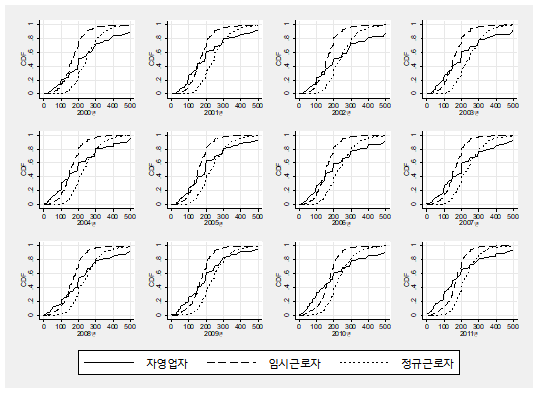
\includegraphics[width=\textwidth]{figure/goms_cdf_myjob.png}
    \label{fig:goms_cdf_myjob}
\end{figure}

 <그림 \ref{fig:goms_cdf_myjob}>은 각각의 코호트에서 직업지위별 소득의 누적분포를 그린 그림이다.
 임시근로자와 정규근로자의 누적분포는 서로 교차없이 정규근로자의 분포가 우하단에 위치하여 임의의 소득을 기준으로 정규근로자가 임시근로자에 대하여 우위에 있다.
  자영업자의 분포를 살펴보면 150만원 이하의 소득에서는 임시근로자보다  좌상단에 있어 불리한 반면 300만원 이상의 소득에서는 정규근로자보다 우하단에 오히려 유리한 모습을 보였다.
 
\section{대학입학의 기회불평등}
먼저 대학입학의 기회불평등 분석결과를 제시한다.
개별 코호트에서 환경유형별 누적분포를 제시하여 개별 환경유형이 획득한 성취의 대략적인 형태를 살펴본다.
 이어서 확률지배검증을 통해 기회불평등의 존재여부를 판단한다.
 지니기회불평등지수를 통해 전반적인 기회불평등 정도의 추이를 살펴보고, 이를 성별 및 입시유형별로 나누어 계산한 값을 통해 소집단에서 집단내 기회불평등의 형태도 아울러 살펴본다.
 마지막으로 개천용불평등지수를 이용하여, 불리한 환경에 속한 개인들이 뛰어난 성취를 획득하는데 있어 기회불평등의 정도를 살펴본다.

\subsection{누적분포함수}
누적분포함수는 총 네 가지 환경 가운데 주성분분석환경과 출신고교지역 두 가지만 제시한다.
\footnote{부모소득환경 및 부모학력환경은 주성분분석환경과 유사한 형태의 분포를 보여 별도로 제시하지 않는다.}
그림 (\ref{fig:goms_cdf_bypca})은 분석 기간인 2000년에서 2011년에 걸쳐 연도별로 가구환경 조건부 대학입학성과의 누적분포를 나타낸 것이다.
주성분분석환경의 누적확률분포는 열악한 환경이 좌상단에 위치하고 유리한 환경이 우하단에 위치하여 전형적인 기회불평등 상황에 놓여있음을 알 수 있다. 

\begin{figure}
    \centering
    \caption{가구환경별 교육성취의 누적분포}
    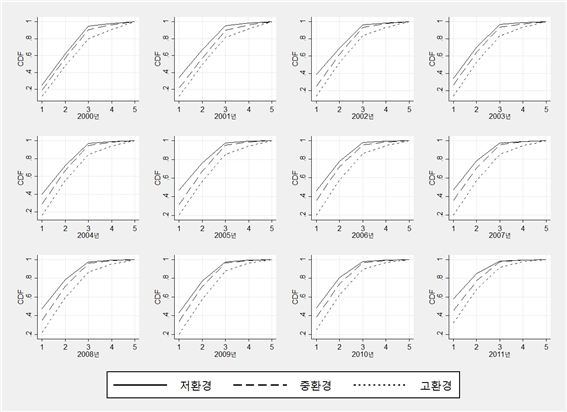
\includegraphics[width=\textwidth]{figure/goms_cdf_bypca.png}
    \label{fig:goms_cdf_bypca}
\end{figure}

출신고교가 위치한 지역에 따른 기회불평등을 확인하기 위해 출신지역을 앞서 설명했던 것처럼 수도권, 광역시, 시군구, 세 가지로 나누고 각 지역구분 별 대학입학성과의 누적분포함수를 도출하여 나타내면 그림 (\ref{fig:goms_cdf_byrgn})와 같다.
출신고교지역 환경에서는 유리한 환경으로 생각한 수도권이 왼쪽 위에 위치하는 경우가 많고 각 환경유형별 함수가 밀접하게 붙어있거나 교차하여 기회불평등이 거의 없는 상황임을 알 수 있다. 

\begin{figure}
    \centering
    \caption{출신지역별 교육성취의 누적분포}
    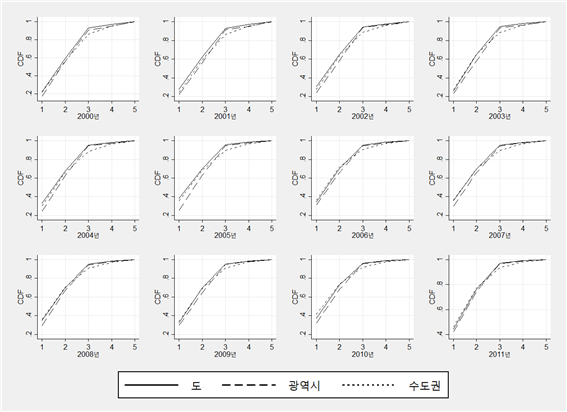
\includegraphics[width=\textwidth]{figure/goms_cdf_byrgn.png}
    \label{fig:goms_cdf_byrgn}
\end{figure}

대학입학에 있어서 성별 기회불평등을 살펴보기 위하여 남성과 여성의 교육성취 누적분포함수를 도출하여 <그림 \ref{fig:goms_cdf_bysex}>에 나타내었다.
남녀의 성비가 어느 정도 균형을 가진 2005년에서 2009년까지의 누적분포함수들을 비교할 때, 모든 연도에서 남성의 누적분포가 여성의 누적분포를 확률지배하여 성별 기회불평등이 존재하는 것으로 나타난다.
 그러나 그 격차는 가구환경별 누적분포의 격차에 비해 뚜렷하지는 않다. 특히 4-5점의 상위권 대학 진학률에서 격차가 작은 것을 알 수 있다.
 
\begin{figure}
    \centering
    \caption{성별 교육성취의 누적분포}
    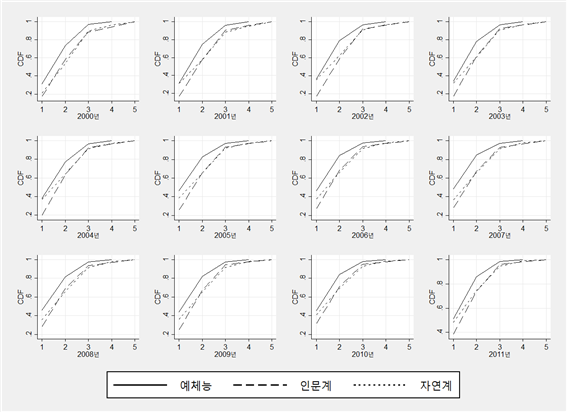
\includegraphics[width=\textwidth]{figure/goms_cdf_bysex.png}
    \label{fig:goms_cdf_bysex}
\end{figure}

마지막으로 대학계열별 교육기회불평등의 존재 유무를 살펴보기 위하여 계열별로 대학입학 성과의 누적분포를 도출하여 <그림 \ref{fig:goms_cdf_byfld}>에 나타내었다.
예체능계의 경우 대학의 선택의 폭이 협소하여 다른 계열에 비해 대학입학 성과가 낮을 것으로 예상된다.
 실제 이런 예상과 같이 예체능계를 선택할 때 대학입학 성과의 누적분포는 인문계 및 자연계에 비해 확연히 열등한 것으로 나타났다.
 그러나 예체능계의 경우 인문, 자연계와 다르게 학교의 종합적인 순위로 성취수준을 정하는 본 연구의 방법이 학생들의 성취에 대한 객관적인 척도라 할 수 없을 것이다.
 \footnote{ 예를들어 연세대, 고려대 본교에는 미술, 체육계열 단과대가 없고 사범대학에 해당계열 학과가 있다.}
 인문계와 자연계 간에는 대학입학 성과의 누적분포 간에 우열관계는 없는 것으로 보이고 두 누적분포가 거의 구분되지 않는 것으로 나타난다.
 
\begin{figure}
    \centering
    \caption{대학계열별 교육성취의 누적분포}
    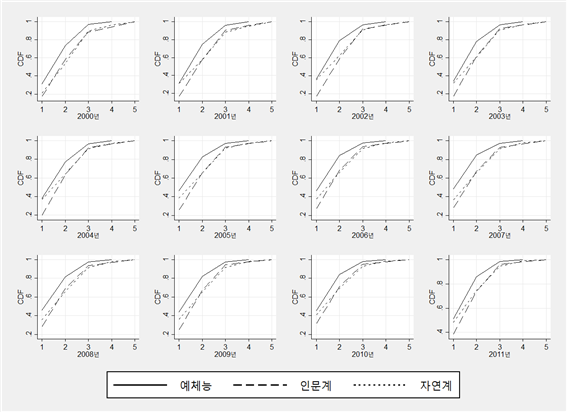
\includegraphics[width=\textwidth]{figure/goms_cdf_byfld.png}
    \label{fig:goms_cdf_byfld}
\end{figure}

\subsection{확률지배결과}

주성분분석 환경하에 확률지배검증 결과 거의 모든 코호트에서 환경유형간에 기회불평등이 존재하는 상황을 확인했다.
특히 대부분의 경우에서 1차 확률지배가 존재하여, 우월한 환경에 속한 수험생들이 평균적으로 좋은 대학에 진학 했음을 알 수 있다.
흥미롭게도 지역의 경우 도 지역과 광역시 사이에서만 일관된 기회불평등이 관찰되는 반면 수도권은 도 지역에 대해서 불분명한 관계인 경우가 많았다.
 광역시와의 비교에서는 오히려 수도권이 확률지배 당하여 이들이 기회불평등 한 경우가 많았는데, 이는 인구가 많은 지역에서 소득 격차가 큰 현상처럼 수도권 학생들의 교육성취 편차가 큰 탓이라고 생각할 수 있다.
 
\begin{table}[htbp]
    \centering
    \caption{PCA환경하 대학입학성과 누적분포의 확률지배 검증결과}
    \begin{tabular}{c|c|c|c|c|c|c}
\hline & \multicolumn{3}{|c|}{중환경} & \multicolumn{3}{c}{고환경} \\
\hline \multirow{4}{*}{저환경} & $<_{1}^{* * *}$ & $<_{1}^{* * *}$ & $<_{1}^{* * *}$ & $<_{1}^{* * *}$ & $<_{1}^{* * *}$ & $<_{1}^{* * *}$ \\
\cline{2-7} & $<_{1}^{* * *}$ & $<_{1}^{* *}$ & $<_{1}^{* * *}$ & $<_{1}^{* * *}$ & $<_{1}^{* * *}$ & $<_{1}^{* * *}$ \\
\cline{2-7} & $<_{1}^{* * *}$ & $<_{1}^{* *}$ & $<_{1}^{* * *}$ & $<_{1 }^{* * *}$ & $<_{1 }^{* * *}$ & $<_{1 }^{* * *}$ \\
\cline{2-7} & $<_{2}^{* * *}$ & $<_{1}^{* * *}$ & $<_{2}^{* * *}$ & $<_{1}^{* * *}$ & $<_{1}^{* * *}$ & $<_{1}^{* * *}$ \\
\hline \multirow{4}{*}{중환경} & 2000 & 2001 & 2002 & $<_{1}^{* * *}$ & $<_{1}^{* * *}$ & $<_{1}^{* * *}$ \\
\cline{2-7} & 2003 & 2004 & 2005 & $<_{1}^{* * *}$ & $<_{1}^{* * *}$ & $<_{1}^{* * *}$ \\
\cline{2-7} & 2006 & 2007 & 2008 & $<_{1}^{* * *}$ & $<_{1}^{* * *}$ & $<_{1}^{* * *}$ \\
\cline{2-7} & 2009 & 2010 & 2011 & $<_{1}^{* * *}$ & $<_{1}^{* * *}$ & $<_{1}^{* * *}$ \\
\hline
\end{tabular}
    \\
    \confer{집단별 상하위 5\%를 각각 제외하고 검증. $=$ 은 동일한 확률분포, $<_{1}$은 행이 열에 1차 확률지배, $<_{2}$는 행이 열에 2차 확률지배 당하는 관계,  $?$는 확률지배관계를 확인 불가능한 경우임. ($*: \alpha = 0.5, **: \alpha = 0.01, ***: \alpha = 0.001$.)}
    \label{tab:goms_dom_bypca}
\end{table}

광역시와 시군구 지역 간에는 전 기간에 걸쳐 뚜렷한 제1차 확률지배관계(광역시가 시군구 환경을 확률지배)가 존재하는 것으로 보이나 광역시와 수도권 그리고 시군구와 수도권 간의 확률지배관계는 뚜렷하지 않다.
 수도권 지역이 대학입학 성과에 우월하다는 통념과 다소 거리가 있는 것으로 보인다.
 그러나 대학의 점수화된 등급을 기준으로 볼 때 3점 이상의 ``상위권 대학'' 진학 확률에 있어서는 전 기간에 걸쳐 수도권 지역이 광역시 혹은 시군구 지역보다 우월한 것으로 나타나고 있어서 수도권 선호의 근거를 보여준다고 할 수 있다.  

\begin{table}[htbp]
    \centering
    \caption{지역별 대학입학성과 누적분포의 확률지배 검증결과}
    \begin{tabular}{c|c|c|c|c|c|c}
\hline & \multicolumn{3}{|c|}{중환경} & \multicolumn{3}{c}{고환경} \\
\hline \multirow{4}{*}{저환경} & $<_{1}^{* * *}$ & $\prec_{1}^{* *}$ & $<_{2}^{* * *}$ & $? ?$ & $<_{1}^{* * *}$ & $<_{1}^{*}$ \\
\cline{2-7} &$<_{1}^{* *}$ & $<_{2}^{* * *}$ & $<_{1 *}^{* *}$ & $? ?$ & $<_{1}^{*}$ & $<_{1}^{*}$ \\
\cline{2-7} &$<_{1}^{*}$ & $<_{2}^{* * *}$ & $<_{2}^{* * *}$ & $? ?$ & $? ?$ & $? ?$ \\
\cline{2-7} &$<_{2}^{* * *}$ & $<_{2}^{* * *}$ & $\prec_{2}^{* *}$ & $? ?$ & $? ?$ & $? ?$ \\
\hline \multirow{4}{*}{중환경} & 2000 & 2001 & 2002 & $? ?$ & $? ?$ & $? ?$ \\
\cline{2-7} & 2003 & 2004 & 2005 & $>_{2}^{* * *}$ & $? ?$ & $>_{2}^{* * *}$ \\
\cline{2-7} & 2006 & 2007 & 2008 & $>_{2}^{* * *}$ & $>_{2}^{* *}$ & $>_{2}^{* * *}$ \\
\cline{2-7} & 2009 & 2010 & 2011 & $>_{2}^{* *}$ & $>_{2}^{* * *}$ & $? ?$\\
\hline
\end{tabular}
    \\
    \confer{집단별 상하위 5\%를 각각 제외하고 검증. $=$ 은 동일한 확률분포, $<_{1}$은 행이 열에 1차 확률지배, $<_{2}$는 행이 열에 2차 확률지배 당하는 관계,  $?$는 확률지배관계를 확인 불가능한 경우임. ($*: \alpha = 0.5, **: \alpha = 0.01, ***: \alpha = 0.001$.)}
    \label{tab:goms_dom_byrgn}
\end{table}

 확률지배 검증을 통하여 전 기간에 걸쳐 광역시지역이 시군구지역을 확률지배한다는 결과를 얻었지만 수도권과 다른 지역 간에는 일관된 확률지배관계가 얻어지지는 않았다.
 2005년에서 2010년에 걸쳐서 광역시지역이 수도권지역을 확률지배한다는 결과는 다소 예상 밖이라 할 수 있다.
  그러나 3점 이상의 상위권 대학에 국한한다면 이러한 확률지배관계가 유지되지는 않을 것으로 보인다.
  수도권과 시군구지역 간의 확률지배관계도 여러 연도에서 확인되지 않는 것도 다소 의외의 결과이다.
  이 경우도 상위권 대학에 국한한다면 수도권의 우위가 나타날 것으로 보인다. 


\subsection{교육성취의 지니기회불평등지수 분석결과}

첫째, 환경별 GOI의 결과부터 살펴본다.
어떤 환경을 선택하느냐에 따라 불평등지수의 크기와 경향이 상이함을 알 수 있다.
 기회불평등 정도는 PCA, 학력, 소득, 지역 순으로 높게 측정된다.
 부모의 학력을 환경으로 했을 경우가 부모의 소득을 환경으로 했을 때보다 일관되게 높은 점은 교육성취 또는 경제력성취의 기회불평등을 대상으로 한 다른 연구와 동일한 결과다.
 주성분분석과 학력 환경의 경우 지수 값의 크기와 성향이 매우 유사하여, 교육성취의 기회불평등이 부모의 학력에서 주로 기인함을 알 수 있다.
 모든 환경변수 하에서 2000년대 중반까지 기회불평등이 상승하는 추세를 보였다가 2008년부터 하락하는 모습을 보인다.
 지역에 의한 기회불평등은 앞서 살펴본 바에서 예상한 바와 같이 매우 낮은 수준이다.

\begin{figure}
    \centering
    \caption{가구환경간 대학입학성과의 지니기회불평등도 추세}
    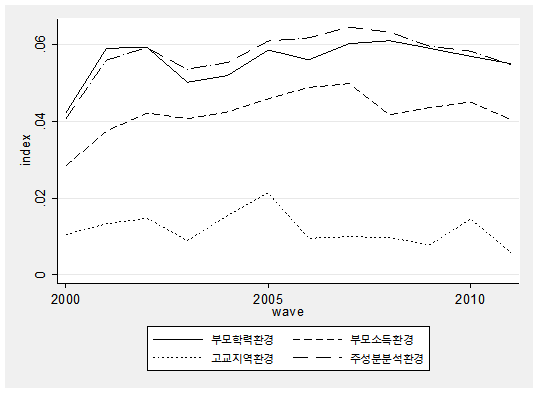
\includegraphics[width=\textwidth]{figure/goms_goi_byenv.png}
    \label{fig:goms_goi_byenv}
\end{figure}

환경-입시유형별 GOI 지수를 살펴본다.
PCA, 학력, 소득의 세 환경에서 일반수시 입학자들 간의 기회불평등이 일반정시 입학자들 간의 기회불평등보다 항상 높았다.
 이는 수시가 정시보다 기회불평등한 대입전형이라는 대중의 인식을 구체적으로 입증한 것이다.
 두 전형간 지수의 격차는 일반정시의 기회불평등이 높아지는 형태도 줄어들고 있어, 정시가 수시에 비해 상대적으로 기회평등했다고 해도 정시제도 자체가 기회평등하지는 않다는 점을 명심해야 한다.
 지역환경에서 기회불평등은 앞서의 환경과 다른 모습이다.
 일반수시에 의한 기회불평등은 2003년부터 꾸준히 감소해 2005년부터는 일반정시보다 현저히 낮다.
 이는 도시 이외지역의 고교가 내신획득에 유리하다는 점과 지역균형선발과 같은 직접적인 지역기회불평등 해소제도의 역할이 작용한 결과로 해석된다.

\begin{figure}
    \centering
    \caption{가구환경간 대학입학성과의 지니기회불평등도 추세: 입시유형별 비교}
    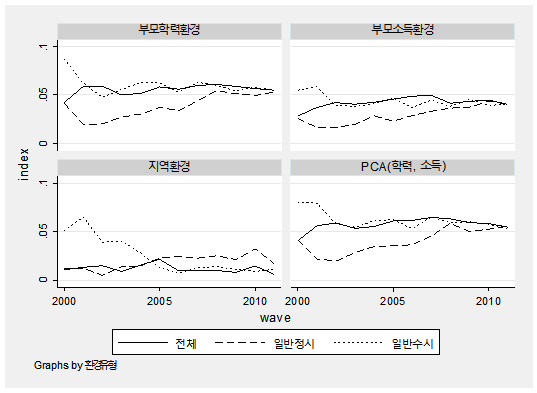
\includegraphics[width=\textwidth]{figure/goms_goi_byent.png}
    \label{fig:goms_goi_byent}
\end{figure}

\subsection{교육성취의 개천용기회불평등지수 분석 결과}
지금부터는 개천용기회불평등지수(RRI)를 살펴본다.
먼저 5점 척도에 의한 환경별 개천용지수의 추이부터 살펴본다.
 RRI에서 지수의 크기는 GOI와 마찬가지로 PCA, 학력, 소득, 지역 순으로 나타났다.
 연도마다 지수의 변동 폭이 커 보이는 데 이는 성공의 기준점이 상위 약 2.8\%로 극히 적은 수를 대상으로 하기 때문이다.
  PCA와 학력을 기준으로 했을 때 평균 약 0.7의 수치를 보이는데, 최우수 대학 및 학과에 진학함에 있어 심각한 기회불평등이 존재함을 알 수 있다.
  부모소득을 환경으로 하면 평균 약 0.6으로 여전히 큰 기회불평등이 존재하지만, PCA나 학력에 비해 상대적으로 낮은 것으로 나타났다.
  출신고교지역을 환경으로 할 경우는 지수는 평균 약 0.3으로 다른 환경들에 비해 현저히 낮고 그 정도도 크게 심각하지 않다.
 
\begin{figure}
    \centering
    \caption{가구환경간 대학입학성과의 개천용기회불평등도 추세}
    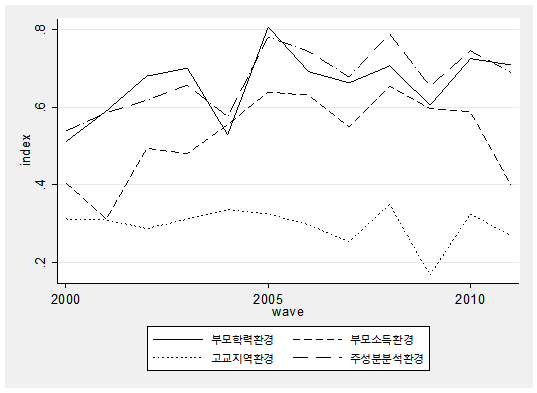
\includegraphics[width=\textwidth]{figure/goms_rri_byenv.png}
    \label{fig:goms_rri_byenv}
\end{figure}

남성 간-여성 간 RRI 차이는 앞서 GOI의 경우와 마찬가지로 차이가 비해 적다.
GOI와는 다르게 부모 학력, 부모소득, 고교지역, PCA의 모든 환경에서는 여성의 기회불평등이 남성보다 다소 높다.
특히 지역 환경에서 경우 다른 환경에 비해 남성 간과 여성 간의 불평등지수의 격차가 가장 크게 나타났다.
여성의 경우 도 지역에서 명문대 및 의대가 있는 도시와 같은 다른 지역으로 유학을 가야 하는 점에 대한 부담감이 작용할 가능성이 있다.


\begin{figure}
    \centering
    \caption{가구환경간 대학입학성과의 개천용기회불평등도 추세: 성별 비교}
    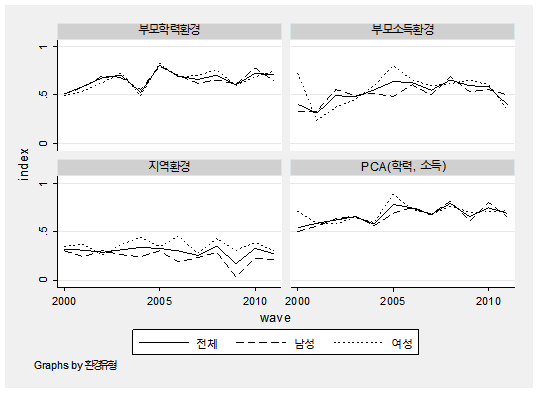
\includegraphics[width=\textwidth]{figure/goms_rri_bysex.png}
    \label{fig:goms_rri_bysex}
\end{figure}

환경-입시유형별 RRI는 GOI 경우와 동일하게 정시보다 수시가 기회불평등 한 것으로 보인다.
특히 지역 환경에서 정시, 수 시간의 격차가 다른 환경보다 매우 크게 나타난다.
 앞서 살펴본 지니기회불평등지수와 환경, 환경-성별 개천용기회불평등지수의 모든 경우에서 지역 환경은 기회불평등 정도가 다른 환경에 비해 현저히 낮고 그 세부구분에서도 차이가 없었다.
 반면 학생이 수시입학을 통해 최상위 교육성취를 얻는데 거주지역이 그 자체로 상당한 기회불평등을 일으키는 것으로 나타났다.
 해당 최상위 대학들의 수시 비중이 높다는 점을 고려했을 때, 이들의 지역균형전형이 충분하지 않음을 짐작할 수 있다.
 2000년과 2001년은 지수 값이 1인 경우가 나오는데 2002년 이후부터 수시정원이 확대되기 시작한 사실과 정시 대 수시 비율이 10:1인 점을 감안하여 예외적인 경우로 보는 것이 타당하다.

\begin{figure}
    \centering
    \caption{가구환경간 대학입학성과의 개천용기회불평등도 추세: 입시유형별 비교}
    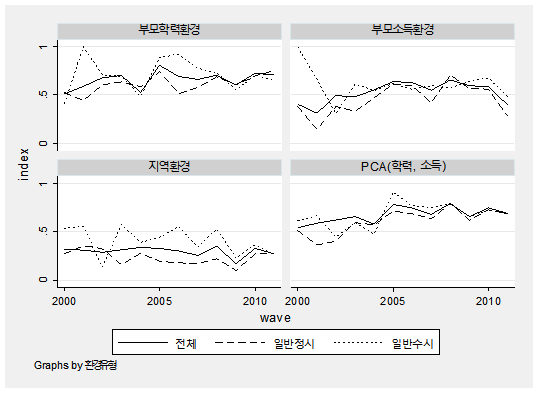
\includegraphics[width=\textwidth]{figure/goms_rri_byent.png}
    \label{fig:goms_rri_byent}
\end{figure}


\section{대학졸업 후 경제적 성취의 기회불평등}
지금부터는 조사대상의 소득의 기회불평등을 분석한다.
모든 취업자를 대상으로 분석하는 경우는 졸업 직후의 경제적 기회불평등을 분석하는데 의의가 있는 반면, 정규근로자 및 자영업자로 제한하여 분석을 하는 것은 조사대상의 향후 소득의 기회불평등 전망에 더 유의미한 자료가 된다.
누적분포 및 확률지배관계 결과는 모든 직업만을 대상으로 진행하였으며, 지수도출은 두 경우를 각각 제시한다.

\subsection{누적분포함수}
앞서와 마찬가지로 주성분분석과 출신고교지역 두 가지 환경에 대한 누적분포를 제시한다.
주성분분석환경에서는 유리한 환경일수록 소득분포가 오른쪽 또는 아래쪽에 위치하여 소득획득에 평균적으로 유리할 것을 알 수 있다.
출신고교지역의 경우는 환경유형별 분포가 거의 유사하여 출신 지역에 의한 소득의 기회불평등이 미미할 것이라고 짐작할 수 있다.
두 환경 모두에서 환경유형간 분포의 차이가 줄어드는 것으로 보여 전반적인 기회불평등도가 감소추세임을 유추할 수 있다.

\begin{figure}
    \centering
    \caption{코호트별 주성분분석환경하 소득의 누적분포}
    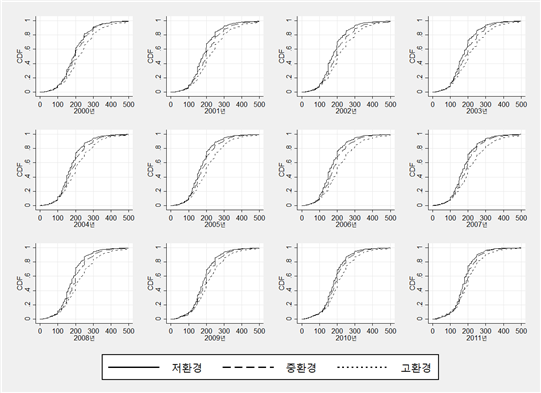
\includegraphics[width=\textwidth]{figure/gomse_cdf_bypca.png}
    \label{fig:gomse_cdf_bypca}
\end{figure}

\begin{figure}
    \centering
    \caption{코호트별 출신고교지역환경하 소득의 누적분포}
    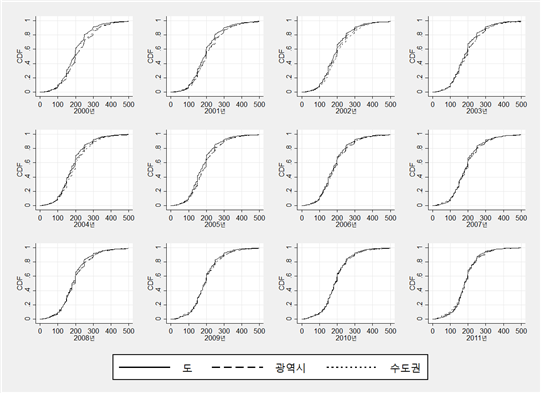
\includegraphics[width=\textwidth]{figure/gomse_cdf_byrgn.png}
    \label{fig:gomse_cdf_byrgn}
\end{figure}

\subsection{확률지배결과}
소득의 경우 분포의 양극단, 다시 말해 매우 낮은 소득이나 매우 높은 소득의 범주에서 환경 간에 분포가 교차하는 경우가 자주 발생한다.
그 결과 자료의 전반에서 확률지배관계가 존재하더라도 없는 것처럼 보이게 한다.
따라서 검증구간에 일부 제한을 두는 것이 필요한데, 본 분석에서는 대부분 자료를 포함할 수 있는 월평균소득 100만 원에서 400만 원 사이의 경우에 대하여 확률지배검증을 시행했다.

\begin{table}[htbp]
    \centering
    \caption{PCA환경하 소득 누적분포의 확률지배 검증결과}
    \begin{tabular}{c|c|c|c|c|c|c}
\hline & \multicolumn{3}{|c|}{중환경} & \multicolumn{3}{c}{고환경} \\
\hline \multirow{4}{*}{저환경} & $=$ & $<_{1}^{**}$ & $<_{1}^{***}$ & $<_{1}^{***}$ & $<_{1}^{***}$ & $<_{1}^{***}$ \\
\cline{2-7} & $<_{2}^{*}$ & $?$ & $<_{1}^{*}$ & $<_{1}^{***}$ & $<_{1}^{***}$ & $<_{1}^{***}$ \\
\cline{2-7} & $<_{2}^{*}$ & $=$ & $<_{2}^{**}$ & $<_{1 }^{***}$ & $<_{1 }^{***}$ & $<_{1 }^{***}$ \\
\cline{2-7} & $=$ & $?$ & $?$ & $<_{1}^{***}$ & $<_{1}^{***}$ & $<_{1}^{***}$ \\
\hline \multirow{4}{*}{중환경} & 2000 & 2001 & 2002 & $<_{1}^{***}$ & $<_{1}^{*}$ & $<_{1}^{***}$ \\
\cline{2-7} & 2003 & 2004 & 2005 & $<_{1}^{***}$ & $<_{1}^{**}$ & $<_{1}^{***}$ \\
\cline{2-7} & 2006 & 2007 & 2008 & $<_{1}^{***}$ & $<_{1}^{***}$ & $<_{1}^{**}$ \\
\cline{2-7} & 2009 & 2010 & 2011 & $<_{1}^{***}$ & $<_{1}^{***}$ & $?$ \\
\hline
\end{tabular}
    \\
    \confer{집단별 상하위 5\%를 각각 제외하고 검증. $=$ 은 동일한 확률분포, $<_{1}$은 행이 열에 1차 확률지배, $<_{2}$는 행이 열에 2차 확률지배 당하는 관계,  $?$는 확률지배관계를 확인 불가능한 경우임. ($*: \alpha = 0.5, **: \alpha = 0.01, ***: \alpha = 0.001$.)}
    \label{tab:gomse_dom_bypca}
\end{table}

주성분분석 환경하에 확률지배검증 결과 거의 모든 연도에서 모든 환경 쌍에 기회불평등이 존재하는 상황을 확인했다.
고환경은 저, 중환경에 대하여 뚜렷하게 확률지배를 하는 것을 확인했다.
반면, 저환경과 중환경 사이에는 동일분포로 판단되는 경우도 있었다.
소득의 기회불평등은 고환경만 절대적으로 유리한 형태로 존재함을 확인했다.
지역의 경우 누적분포함수에서 유추할 수 있듯이 거의 모든 환경 유형의 쌍에서 확률지배검증이 안 되거나 동일분포로 판단되어 출신고교지역에 의한 소득의 기회불평등은 거의 없는 것을 확인했다.

\begin{table}[htbp]
    \centering
    \caption{PCA환경하 소득 누적분포의 확률지배 검증결과}
    \begin{tabular}{c|c|c|c|c|c|c}
\hline & \multicolumn{3}{|c|}{중환경} & \multicolumn{3}{c}{고환경} \\
\hline \multirow{4}{*}{저환경} & $?$ & $?$ & $=$ & $?$ & $?$ & $<_{1}^{***}$ \\
\cline{2-7} & $?$ & $<_{2}^{**}$ & $?$ & $?$ & $<_{1}^{*}$ & $?$ \\
\cline{2-7} & $=$ & $?$ & $?$ & $=$ & $?$ & $?$ \\
\cline{2-7} & $=$ & $=$ & $?$ & $?$ & $=$ & $?$ \\
\hline \multirow{4}{*}{중환경} & 2000 & 2001 & 2002 & $=$ & $=$ & $<_{2}^{***}$ \\
\cline{2-7} & 2003 & 2004 & 2005 & $=$ & $?$ & $?$ \\
\cline{2-7} & 2006 & 2007 & 2008 & $=$ & $=$ & $=$ \\
\cline{2-7} & 2009 & 2010 & 2011 & $=$ & $=$ & $=$\\
\hline
\end{tabular}
    \\
    \confer{집단별 상하위 5\%를 각각 제외하고 검증. $=$ 은 동일한 확률분포, $<_{1}$은 행이 열에 1차 확률지배, $<_{2}$는 행이 열에 2차 확률지배 당하는 관계,  $?$는 확률지배관계를 확인 불가능한 경우임. ($*: \alpha = 0.5, **: \alpha = 0.01, ***: \alpha = 0.001$.)}
    \label{tab:gomse_dom_byrgn}
\end{table}

\subsection{소득의 지니기회불평등지수 분석 결과}
환경별 GOI의 추이는 PCA와 부모소득이 거의 동일하고, 부모학력, 지역 순으로 높게 측정된다.
모든 환경에 대하여 GOI의 값이 거의 절반 수준에 머물러, 교육의 성취보다 소득에서 환경의 영향이 훨씬 낮음을 알 수 있다.
앞서 교육성취와는 다르게 주성분분석과 소득환경의 경우가 지수 값의 크기와 성향이 매우 유사하여, 소득성취의 기회불평등은 부모의 소득에서 주로 기인함을 알 수 있다.
모든 환경변수 교육성취에서는 2008년부터 지수의 전반적인 하락세가 있었는데 소득에서는 한 해 빠른 2007년부터 하락세가 보인다.
지역에 의한 기회불평등은 역시 거의 없는 수준이다.
모든직업을 대상으로 할 경우보다 정규직$\cdot$자영업을 대상으로 할 경우의 불평등도가 높게 나오는데, 이는 정규직이라는 우월한 직위를 획득하는데 대한 기회불평등 역시 존재함을 반영한다.

\begin{figure}
    \centering
    \caption{환경별 소득의 지니기회불평등지수 추이}
    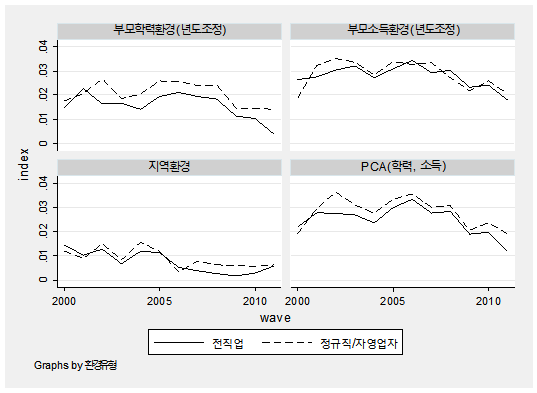
\includegraphics[width=\textwidth]{figure/gomse_goi_byenv.png}
    \label{fig:gomse_goi_byenv}
\end{figure}

환경-입시유형별 GOI 지수는 <그림 \ref{fig:goms_goi_byent}>에 나타나 있다.
정규직$\cdot$자영업자의 경우 48개 조사시점 가운데 총 38개 조사시점에서 일반수시 졸업자간의 기회불평등이 일반정시 졸업자간의 기회불평등보다 유의미하게 높았다.
이는 매우 흥미로운 결과인데 입시제도가 대학입학에 일시적인 영향을 주는 것을 넘어서 졸업 이후의 소득획득에도 관계가 있다고 해석할 수 있다.
하지만 대입유형은 수험생들이 선택할 수 있고 정시와 수시의 정원은 수험생들과 무관하게 바뀌고 있는 등의 요소에 대한 통제가 없는 본 연구에서 특정 대입제도가 미래 개인들의 소득획득에 인과관계가 존재한다고 이야기 할 수 없다.

\begin{figure}
    \centering
    \caption{환경-대입유형별별 소득획득의 개천용불평등지수 추이}
    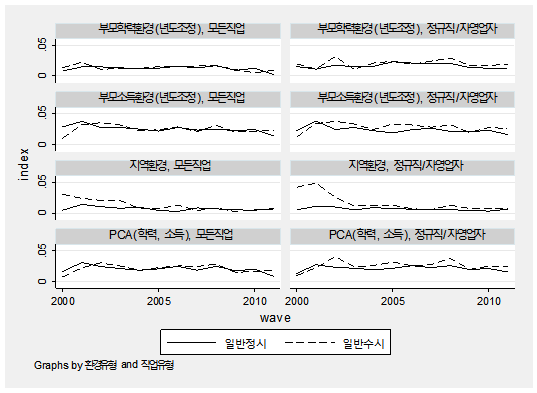
\includegraphics[width=\textwidth]{figure/gomse_goi_byent.png}
    \label{fig:gomse_goi_byent}
\end{figure}

\subsection{소득의 개천용기회불평등지수 분석 결과}
지금부터는 개천용기회불평등지수(RRI)를 통해 고소득 획득에서 기회불평등 양상을 살펴본다.
 앞서 대학입학의 경우 최상위인 5점을 성공의 척도로 삼았는데, 이들은 상위 약 2.8\% 이었다.
 대학입학과 결과 비교를 위해 소득에서도 상위 2.8\%를 성공의 기준으로 한다.
 하지만 소득 2.8\%는 성공의 기준으로 지나치게 엄격하다.
 또한 불리한 환경에서 성공하는 개인의 수가 현저히 줄어들어 개천용불평등지수 표준오차가 과대 측정되고, 남녀간 또는 대입유형간 지수비교에서 유의성이 현저히 감소할 수 있다.
 그래서 또다른 성공의 기준으로 소득 상위 10\%를 이용한 지수값을 같이 제시한다.
 
\begin{figure}
    \centering
    \caption{환경별 소득의 개천용기회불평등지수 추이: 상위 2.8\% 성공기준}
    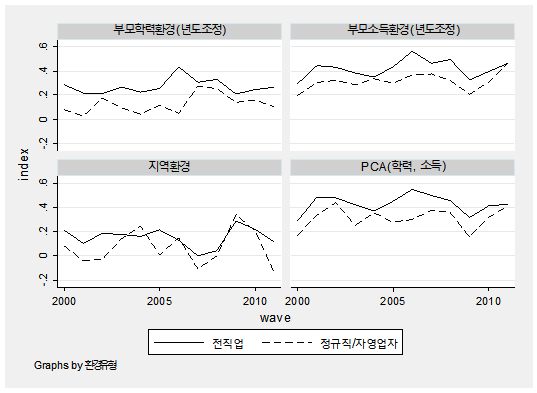
\includegraphics[width=\textwidth]{figure/gomse_rri_byenv_28.png}
    \label{fig:gomse_rri_byenv_28}
    \confer{성공기준은 코호트별 소득 상위 2.8\%.}
\end{figure}

 <그림 \ref{fig:gomse_rri_byenv_28}>는 상위 2.8\%소득을 성공의 기준으로 한 RRI의 추이다.
 GOI의 경우 대학입학을 성취로 했을 경우에 비하여 소득을 성취로 한 지수값이 거의 절반 가깝게 하락했던 반면 RRI에서는 지수값은 하락하지만 하락폭은 GOI에 비해 크지않은 것을 알 수 있다.
 환경별로는 GOI와 마찬가지로 PCA 및 소득, 학력, 지역 순으로 나타났다.
 PCA 소득을 환경으로 했을 때 약 지수 값이 0.4 근처에 있어, 불리한 환경에 속한 개인들은 10명 중 4명은 환경의 영향으로 상위 2. 8\% 소득의 획득에 실패한다고 할 수 있다.
 하지만 0.6-0.7 사이에 위치하는 대학입학의 지수 값과 비교한다면 불평등의 정도가 현저히 낮음을 알 수 있다.
 지역의 경우 음의 지수값이 나오는 코호트가 있는데 이는 도지역 출신자가 전체 인구에서의 비율보다 소득상위 2.8\%에서 더 많이 존재한다는 의미로 지역환경은 정규직/자영업자의 고소득 획득에 불리한 영향을 거의 주지 않음을 알 수 있다.

\begin{figure}
    \centering
    \caption{환경별 소득의 개천용기회불평등지수 추이: 상위 10\% 성공기준}
    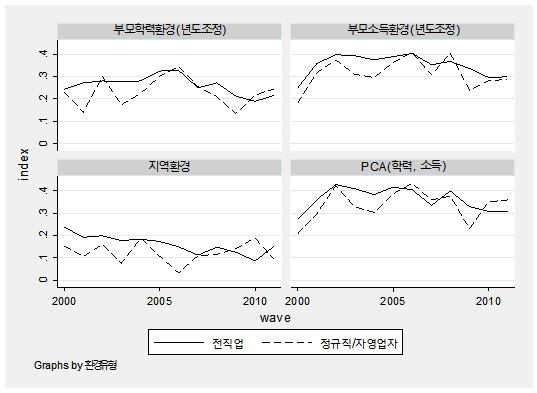
\includegraphics[width=\textwidth]{figure/gomse_rri_byenv_10.png}
    \label{fig:gomse_rri_byenv_10}
\end{figure}

상위 10\% 소득을 성공기준으로 하는 <그림 \ref{fig:gomse_rri_byenv_10}>는 완화된 성공의 기준으로 인해 <그림 \ref{fig:gomse_rri_byenv_28}>보다 수치가 전반적으로 낮다.
 전직업의 경우 코호트별 지수의 변동폭이 줄어드는 반면 정규직$\cdot$자영업자는 변동폭이 늘어나는 상반된 모습을 보였다.
 GOI의 경우 2009-2011년 코호트에서 하락하는 추세였으나 RRI에서는 두 성공기준 모두에서 상승하는 양상을 나타냈다.
 이는 성공기준에 속하는 인원 가운데 열악한 환경에 속한 개인들의 수는 줄어든 반면 중간 환경에 속한 개인들의 수가 크게 늘었기 때문이다.

\begin{figure}
    \centering
    \caption{환경별 소득의 개천용기회불평등지수 추이: 상위 10\% 성공기준}
    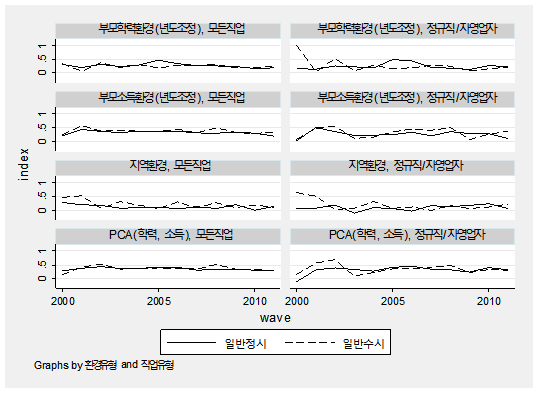
\includegraphics[width=\textwidth]{figure/gomse_rri_byent_10.png}
    \label{fig:gomse_rri_byent_10}
\end{figure}

환경-입시유형별 RRI는 GOI 경우와 특정한 입시유형이 성공에서 더 기회불평등한 경우는 없다.
 <그림 \ref{fig:gomse_rri_byent_10}>을 보면 일반정시와 일반수시의 추이가 대부분의 경우에서 수시로 교차하는 것을 확인할 수 있다.
 2000년과 2001년은 대학입학의 경우와 마찬가지로 수시로 합격한 개인이 적은 탓에 유의미한 결과가 아닌 것으로 해석해야 한다.

\section{소결론 및 시사점}

가구의 사회경제적 지위에 따라 대학진학 성과 및 생애 첫 소득의의 기회불평등이 조사 기간 전체에 걸쳐 뚜렷하게 존재하는 것으로 나타났다.
지역에 따른 성취의 기회불평등은 대학진학 및 소득 모두에서 불분명하지만, 광역시와 시군구 간의 기회불평등은 대학진학에서 뚜렷하게 나타났다.

대학진학에서 지니기회불평등지수는 2007년을 전후로 완만한 상승에서 완만한 하강으로 바뀐다.
 개천용기회불평등지수는 2007년 이후에도 상승세를 보였고, 특히 수준이 매우 높아 조사 기간 말에는 열악한 환경에서 기회불평등으로 최상위권 대학진학에 실패할 확률이 70\%에 이르는 것으로 나타났다.
 입시 전형별로 일반수시 합격자간 기회불평등이 일반정시 합격자간 기회불평등보다 높은 것으로 나타났다.
 그러나 일반정시 합격자간 기회불평등도는 조사 기간에 걸쳐 꾸준히 상승하여 수시와 정시 간의 기회불평등도 격차는 크게 줄어들었다.
 이러한 현상이 정시 비중이 2002년 70\%에서 2019년 현재 40\%대로 감소하는 상황과 관련된 것인지에 대하여 추가적인 연구가 필요하다.

소득의 경우 대학진학에 비해 기회불평등의 정도가 현저히 낮은 것으로 나타났다.
 소득의 지니기회불평등지수는 2008년 이후부터 완만한 내림세를 보인다.
 개천용기회불평등지수 역시 2007년부터 하락하지만 2009년부터는 다시 상승하는 반대 추세를 보였다.
 대학진학보다는 낮은 수치이지만, 열악한 환경에서 기회불평등으로 고소득 획득에 실패할 확률이 40\%라는 결론은 무시할 수 없는 수치이다.
 입시 전형별로 일반수시로 대학에 들어간 개인들 사이의 기회불평등이 일반정시로 대학에 들어간 개인들 간의 기회불평등보다 유의하게 높았다.
 지니기회불평등 지수로 확인한 입시유형간의 소득획득의 기회불평등은 개천용기회불평등지수로 분석한 고소득 획득에서는 유의미한 차이가 없었다.
 성별의 경우 소득획득에서 명백한 기회불평등이 존재함을 확인했다.

본 연구는 대졸자를 대상으로 하였기 때문에 교육 및 경제적 성취의 기회불평등을 과소 측정하는 문제를 안고 있다.
 특히 1절에서 본것과 같이 열악한 환경일수록 수능에 응시하지 않고 따라서 대학진학 이루어지지 않았기 때문에 열악한 환경에 처한 집단의 성취가 과대측정되는 문제가 있다.

향후 연구과제는 다음과 같다.
본 연구는 성별, 입학유형별로 제한을 통해 정시입학자간, 수시입학자간 기회불평등에 대한 분석은 수행하였다.
 이를 통해 성별과 대입유형이 성취의 기회불평등에 영향을 준다는 점은 확인했다.
 하지만 이러한 요소가 성취와 성취의 기회불평등과 어떤 관련이 있는가에 대한 구체적인 결론은 향후 연구되어야 할 과제다.
 특히 성별에 의해 유발되는 기회불평등의 정도와 대입유형과 소득과의 관계가 그러하다.